\documentclass[twocolumn]{aastex631}

\usepackage{amsmath}
\usepackage{multirow}
\usepackage{natbib}
\usepackage{graphicx} 
\usepackage{aas_macros}


\begin{document}

\title{Quantum Kinetic Structure Preservation in Horndeski Theories: Ensuring One-Loop Stability and Testable Cosmology}

\author{Denario}
\affiliation{Anthropic, Gemini \& OpenAI servers. Planet Earth.}

\begin{abstract}
Horndeski theories, while constructed to be classically ghost-free, face the critical challenge of preserving this stability under quantum corrections, which often introduce problematic higher-derivative ghost terms into the effective action. This paper proposes the Quantum Kinetic Structure Preservation (QKSP) symmetry, a principle defined by specific algebraic and differential relations among the theory's functions, designed to explicitly maintain its intrinsic ghost-free kinetic structure at the one-loop level and prevent the generation of new propagating ghost degrees of freedom. Our multi-stage theoretical analysis first establishes classical stability conditions for Horndeski theories around a flat Friedmann-Lemaître-Robertson-Walker background, incorporating the observational constraint of luminal gravitational wave propagation ($c_T^2=1$). We then compute the one-loop effective action using the background field method and heat kernel regularization to identify quantum-generated higher-derivative terms. The QKSP conditions are derived by demanding the vanishing of coefficients for terms that would introduce higher-than-second-order time derivatives in the effective action for physical perturbations. We find that QKSP symmetry fundamentally implies that scalar and tensor modes must propagate at the same speed ($c_s^2 = c_T^2$), which, combined with the empirical $c_T^2=1$, leads to the strong prediction that QKSP-symmetric Horndeski theories must satisfy $c_s^2=1$. A subsequent phenomenological analysis of a representative QKSP-symmetric model, capable of mimicking the $\Lambda$CDM expansion history, reveals a gravitational slip parameter $\eta=1$ and time-dependent modifications to the effective gravitational constant, $G_{\text{eff}}$. For instance, a coupling parameter $|c_B|=0.1$ predicts percent-level deviations in $G_{\text{eff}}$ (e.g., a 7.4% enhancement or 6.4% suppression at $z=0$) that are within reach of current and future large-scale structure surveys. This work establishes a direct link between fundamental quantum stability requirements and observable cosmological phenomena, presenting a theoretically motivated and observationally falsifiable framework for modified gravity.
\end{abstract}

\keywords{Dark energy, Friedmann-Robertson-Walker metric, Cosmic microwave background radiation, Friedmann universe, Large-scale structure of the universe}


\section{Introduction}
\label{sec:intro}

The current cosmological paradigm, known as the $\Lambda$CDM model, has achieved remarkable success in describing a vast array of astrophysical and cosmological observations, from the cosmic microwave background to the large-scale distribution of galaxies. Despite its empirical triumphs, $\Lambda$CDM relies on the existence of dark energy and dark matter, whose fundamental nature remains one of the most profound mysteries in physics. This unresolved enigma has spurred significant interest in theories of modified gravity, which aim to explain cosmic acceleration and structure formation without resorting to these exotic, unobserved components. Among the diverse landscape of modified gravity theories, scalar-tensor theories, where a dynamically evolving scalar field couples to gravity, offer a rich and well-motivated framework. Within this broad class, Horndeski theories stand out as the most general theories of gravity coupled to a single scalar field that yield second-order equations of motion for both the metric and the scalar field. This crucial property ensures that these theories are classically free from Ostrogradsky ghost instabilities, which would otherwise render them pathological at the classical level. The Horndeski action, defined by specific functions $G_i(\phi, X)$ where $X = -\frac{1}{2}\nabla_\mu\phi \nabla^\mu\phi$, provides a powerful framework for exploring alternatives to $\Lambda$CDM, capable of mimicking dark energy and modifying the growth of cosmic structures.

However, the classical ghost-free nature of Horndeski theories does not automatically guarantee their stability at the quantum level. A fundamental and notoriously difficult challenge in modified gravity theories, and indeed in quantum field theories in curved spacetimes, is the potential for quantum corrections to introduce new, problematic degrees of freedom into the effective action. Specifically, at the one-loop level, the functional integration over quantum fluctuations can generate higher-derivative terms (e.g., terms involving four or more derivatives of the fields) in the effective action. If these higher-derivative terms appear with the wrong sign or structure in the kinetic sector of the effective theory for physical perturbations, they typically lead to the emergence of Ostrogradsky ghosts. These quantum-induced ghosts propagate with negative kinetic energy, causing the vacuum to be catastrophically unstable and rendering the theory physically inconsistent. Ensuring the absence of such quantum ghosts is a critical requirement for any truly viable theory of gravity beyond General Relativity, yet it is a problem made difficult by the complexity of quantum calculations in curved backgrounds and the inherent non-renormalizability of gravity.

This paper proposes a novel and systematic approach to address this profound quantum stability problem: the Quantum Kinetic Structure Preservation (QKSP) symmetry. QKSP symmetry is a principle defined by specific algebraic and differential relations among the Horndeski functions $G_i(\phi, X)$ and their derivatives. Its core purpose is to explicitly ensure that the intrinsic ghost-free kinetic structure of the theory, which holds at the classical level, is rigorously maintained even after accounting for one-loop quantum corrections. In essence, QKSP symmetry dictates that any higher-derivative terms generated in the one-loop effective action for the physical scalar and tensor degrees of freedom are precisely of a form that *do not introduce new propagating ghost degrees of freedom*. This implies a delicate cancellation or specific structuring of quantum-generated terms, preventing the emergence of problematic higher-than-second-order time derivatives in the equations of motion for physical perturbations.

Our investigation proceeds through a multi-stage theoretical and phenomenological analysis. We begin by establishing the classical stability conditions for Horndeski theories around a flat Friedmann-Lemaître-Robertson-Walker (FLRW) background, analyzing both tensor and scalar perturbations. A crucial observational constraint, the luminal propagation of gravitational waves ($c_T^2=1$), is enforced from the outset, significantly simplifying the Horndeski action by constraining the functions $G_4$ and $G_5$. The central part of our work involves the rigorous computation of the one-loop effective action using the background field method and heat kernel regularization. This systematic calculation allows us to identify the quantum-generated higher-derivative terms that could potentially introduce ghosts. The QKSP conditions are then derived by demanding the precise vanishing of the coefficients of any terms in the effective action that would lead to higher-than-second-order time derivatives for the physical perturbations, thereby ensuring the preservation of the kinetic structure.

A striking and fundamental consequence of QKSP symmetry, when combined with the observational constraint $c_T^2=1$, is the strong prediction that scalar modes must also propagate at the speed of light, i.e., $c_s^2=1$. This establishes a direct and powerful link between fundamental quantum stability requirements and the propagation speeds of cosmological perturbations. Finally, we verify the cosmological viability of a representative QKSP-symmetric model, capable of mimicking the $\Lambda$CDM expansion history. Our phenomenological analysis focuses on the behavior of linear perturbations, specifically computing the effective gravitational constant, $G_{\text{eff}}$, and the gravitational slip parameter, $\eta$. We demonstrate that these QKSP-symmetric theories predict characteristic, time-dependent deviations in $G_{\text{eff}}$ (e.g., percent-level enhancements or suppressions) that are within the reach of current and future large-scale structure surveys. This work thus offers a theoretically motivated framework for modified gravity that is not only robustly stable at the quantum level but also makes concrete, falsifiable predictions for observable cosmological phenomena, thereby establishing a direct bridge between fundamental quantum principles and observational cosmology.


\section{Methods}
\label{sec:methods}
Our investigation into the quantum stability and cosmological viability of Horndeski theories proceeds through a multi-stage theoretical and phenomenological analysis. This systematic approach is designed to first establish the classical ghost-free structure of these theories, then rigorously identify the conditions required to preserve this structure at the one-loop quantum level, and finally assess the observational implications of such quantum-stable models.

\subsection{Classical Framework and Stability Analysis}
The foundational step of our methodology involves a detailed analysis of the classical Horndeski action, which represents the most general scalar-tensor theory yielding second-order equations of motion for both the metric and the scalar field. This classical ghost-free property is paramount for any viable gravitational theory. The Horndeski action is given by:
\begin{equation}
S = \int d^4x \sqrt{-g} \sum_{i=2}^{5} \mathcal{L}_i
\end{equation}
where the individual Lagrangian densities $\mathcal{L}_i$ are defined as:
\begin{itemize}
    \item $\mathcal{L}_2 = G_2(\phi, X)$
    \item $\mathcal{L}_3 = G_3(\phi, X) \Box\phi$
    \item $\mathcal{L}_4 = G_4(\phi, X) R + G_{4,X}(\phi, X) [(\Box\phi)^2 - (\nabla_\mu\nabla_\nu\phi)^2]$
    \item $\mathcal{L}_5 = G_5(\phi, X) G_{\mu\nu}\nabla^\mu\nabla^\nu\phi - \frac{1}{6}G_{5,X}(\phi, X) [(\Box\phi)^3 - 3(\Box\phi)(\nabla_\mu\nabla_\nu\phi)^2 + 2(\nabla_\mu\nabla_\nu\phi)^3]$
\end{itemize}
Here, $X = -\frac{1}{2}\nabla_\mu\phi \nabla^\mu\phi$ is the kinetic term of the scalar field $\phi$, and $G_i(\phi, X)$ are arbitrary functions of $\phi$ and $X$.

To assess classical stability, we employ perturbation theory around a flat Friedmann-Lemaître-Robertson-Walker (FLRW) background metric, $ds^2 = -N(t)^2 dt^2 + a(t)^2 \delta_{ij} dx^i dx^j$, coupled to a homogeneous and isotropic scalar field $\phi(t)$. This involves expanding the full action to second order in infinitesimal perturbations of the metric and scalar field. Specifically, we consider tensor perturbations, denoted by $h_{ij}$, and scalar perturbations, typically parametrized by a gauge-invariant variable such as $\zeta$.

\subsubsection{Derivation of Classical Stability Conditions}
The second-order action for these perturbations reveals their kinetic and gradient terms. For a theory to be classically stable, two conditions must be met for each propagating degree of freedom:
\begin{enumerate}
    \item \textbf{No-Ghost Condition}: The kinetic term for the perturbation must have a positive sign. A negative kinetic term indicates the presence of an Ostrogradsky ghost, a pathological degree of freedom with negative energy, rendering the vacuum unstable.
    \item \textbf{No Gradient Instability Condition}: The gradient term for the perturbation must have a positive sign. A negative gradient term implies that perturbations can grow exponentially at short wavelengths, leading to instabilities. The coefficient of the gradient term defines the squared propagation speed of the perturbation ($c_s^2$ for scalar modes, $c_T^2$ for tensor modes), which must be real and non-negative.
\end{enumerate}
The specific conditions derived from this analysis, evaluated on the FLRW background, are summarized below:

\begin{tabular}{|l|l|l|}
\hline
\textbf{Perturbation Type} & \textbf{Stability Condition} & \textbf{Mathematical Requirement on Background Quantities} \\
\hline
Tensor & No-Ghost & $\mathcal{G}_T = 2(G_4 - X G_{4,X} - \frac{1}{2}\dot{\phi} H G_{5,X} + \frac{1}{2}X G_{5,\phi}) > 0$ \\
\hline
Tensor & No Gradient Instability & $c_T^2 = \frac{2G_4 - 2X G_{4,X} - \ddot{\phi} G_{5,X}}{2G_4 - 2X G_{4,X} + \dot{\phi} H G_{5,X} - X G_{5,\phi}} > 0$ \\
\hline
Scalar & No-Ghost & $\mathcal{G}_S = \frac{1}{a^2 H^2} \Sigma \mathcal{G}_T^2 + 3 \mathcal{G}_T > 0$ \\
\hline
Scalar & No Gradient Instability & $c_s^2 = \frac{1}{aH\mathcal{G}_S} \frac{d}{dt}\left( \frac{a}{H} \frac{\mathcal{G}_T^2}{\Sigma} \right) - \frac{\mathcal{F}_T}{\mathcal{G}_S} > 0$ \\
\hline
\end{tabular}

Here, $\Sigma$, $\mathcal{F}_T$, and other background quantities are specific combinations of the Horndeski functions $G_i$ and their derivatives, evaluated on the FLRW background. A crucial observational constraint is the luminal propagation of gravitational waves, $c_T^2=1$, as established by GW170817 and GRB 170817A. Enforcing $c_T^2=1$ from the outset significantly constrains the Horndeski functions, specifically requiring $G_{4,X}=0$ and $G_{5,X}=0$. This simplifies the theory by eliminating certain higher-derivative terms from the classical action, which in turn reduces the complexity of subsequent quantum calculations.

\subsection{One-Loop Effective Action Calculation}
The core of our theoretical analysis is the computation of the one-loop quantum corrections to the Horndeski action. This is crucial for identifying any quantum-generated higher-derivative terms that could introduce problematic ghost degrees of freedom, which is the central challenge addressed by the Quantum Kinetic Structure Preservation (QKSP) symmetry. We employ the background field method combined with heat kernel regularization for this calculation.

\subsubsection{Background Field Method}
The background field method provides a systematic way to compute the effective action by separating the fields into classical background components and quantum fluctuations. For our Horndeski theory, we decompose the metric $g_{\mu\nu}$ and scalar field $\phi$ as:
\begin{align*}
g_{\mu\nu} &= \bar{g}_{\mu\nu} + h_{\mu\nu} \\
\phi &= \bar{\phi} + \delta\phi
\end{align*}
where $\bar{g}_{\mu\nu}$ and $\bar{\phi}$ represent the classical background (specifically, the FLRW solution and its associated scalar field profile), and $h_{\mu\nu}$ and $\delta\phi$ are the quantum fluctuations. The full action $S[g, \phi]$ is then expanded in powers of these fluctuations around the background. The one-loop effective action, $\Gamma^{(1)}[\bar{g}, \bar{\phi}]$, is obtained by functionally integrating over the quantum fluctuations:
\begin{equation}
\exp(i\Gamma^{(1)}[\bar{g}, \bar{\phi}]) = \int \mathcal{D}h \mathcal{D}(\delta\phi) \exp(i S^{(2)}[\bar{g}, \bar{\phi}; h, \delta\phi])
\end{equation}
where $S^{(2)}$ is the quadratic part of the action in terms of the fluctuations. This quadratic action can be written in the generic form $S^{(2)} = \frac{1}{2} \int d^4x \sqrt{-\bar{g}} \Psi_A \Delta^{AB} \Psi_B$, where $\Psi_A$ collectively denotes the fluctuation fields ($h_{\mu\nu}$, $\delta\phi$) and $\Delta^{AB}$ is a differential operator. The functional integral then yields the functional determinant of this operator: $\Gamma^{(1)} = \frac{i}{2} \text{Tr} \log(\Delta)$.

\subsubsection{Heat Kernel Regularization}
The functional determinant $\text{Tr} \log(\Delta)$ is typically divergent and requires regularization. We utilize the heat kernel method, a powerful technique for calculating one-loop effective actions in curved spacetimes. The heat kernel $K(x, y; \tau)$ for an operator $\Delta$ satisfies the heat equation $(\partial_\tau + \Delta) K(x, y; \tau) = 0$ with the initial condition $K(x, y; 0) = \delta(x-y)$. The trace of the logarithm of $\Delta$ can be expressed as an integral over the heat kernel:
\begin{equation}
\text{Tr} \log(\Delta) = -\int_0^\infty \frac{d\tau}{\tau} \text{Tr}_{\text{reg}}[K(\tau)]
\end{equation}
where $\text{Tr}_{\text{reg}}$ denotes a regularized trace. For a generic elliptic operator $\Delta$, the short-time expansion of the heat kernel trace is given by the Seeley-DeWitt expansion:
\begin{equation}
\text{Tr}[K(\tau)] \sim \int d^4x \sqrt{-\bar{g}} \sum_{n=0}^{\infty} a_n(x, \Delta) \tau^{n-2}
\end{equation}
The coefficients $a_n(x, \Delta)$, known as the Seeley-DeWitt coefficients, are local geometric invariants constructed from the background fields and their derivatives. Substituting this expansion into the integral for $\text{Tr} \log(\Delta)$ reveals the divergent terms (corresponding to $n < 2$) and finite terms. The terms of interest for our analysis are those arising from $a_2(x, \Delta)$, as these coefficients generate dimension-four operators in the effective action, including higher-derivative terms that could introduce new kinetic pathologies. Examples of such terms include $R^2$, $R_{\mu\nu}R^{\mu\nu}$, and scalar-tensor analogues like $(\Box\phi)^4$, $(\nabla_\mu\nabla_\nu\phi)^2 (\Box\phi)^2$, etc. The calculation will be systematically performed using dimensional regularization to handle these divergences and extract the finite parts, which contribute to the quantum-corrected action.

\subsection{Derivation of the Quantum Kinetic Structure Preservation (QKSP) Conditions}
The central objective of this research stage is to formulate the Quantum Kinetic Structure Preservation (QKSP) conditions. This principle asserts that the one-loop corrected effective action, $S_{\text{eff}} = S_{\text{classical}} + \Gamma^{(1)}$, must not introduce any new propagating ghost degrees of freedom that were absent at the classical level. Such ghosts would manifest as higher-than-second-order time derivatives in the equations of motion for physical perturbations, leading to classical instabilities.

\subsubsection{Identifying Problematic Higher-Derivative Terms}
Upon computing $\Gamma^{(1)}$ using the heat kernel method, we meticulously identify all terms that involve four or more derivatives of the background fields. These terms can include combinations of Ricci scalars, Ricci tensors, Riemann tensors, and covariant derivatives of the scalar field (e.g., $R^2$, $R_{\mu\nu}R^{\mu\nu}$, $R_{\mu\nu\rho\sigma}R^{\mu\nu\rho\sigma}$, $(\Box\phi)^2 R$, $\nabla_\mu\nabla_\nu\phi \nabla^\mu\nabla^\nu\phi R$, etc.). These are the potential sources of new quantum ghosts.

\subsubsection{Perturbation of the Effective Action and Kinetic Analysis}
The next crucial step is to expand the total effective action $S_{\text{eff}}$ to second order in the physical tensor ($h_{ij}$) and scalar ($\zeta$) perturbations around the FLRW background. This yields the quadratic action for these perturbations, which now includes contributions from both the classical action and the one-loop quantum corrections. We then carefully examine the kinetic sector of this expanded quadratic action.
Specifically, we look for terms proportional to higher powers of time derivatives of the perturbations, such as $(\dddot{h}_{ij})^2$, $(\ddot{\zeta})^2$, $(\nabla^2 \ddot{\zeta})$, etc. The presence of terms involving three or more time derivatives in the equations of motion for $h_{ij}$ or $\zeta$ would indicate the emergence of new Ostrogradsky ghost degrees of freedom, which are incompatible with a stable quantum theory.

\subsubsection{Imposing the QKSP Conditions}
The QKSP conditions are derived by demanding that the coefficients of all such problematic higher-than-second-order time derivative terms in the quadratic action for physical perturbations vanish identically. This requires specific algebraic and differential relations among the original Horndeski functions $G_i(\phi, X)$ and their derivatives. These relations constitute the mathematical definition of the QKSP symmetry. By enforcing these conditions, we ensure that the intrinsic ghost-free kinetic structure of the classical Horndeski theory is rigorously preserved at the one-loop level. A remarkable outcome of this derivation, when combined with the observational constraint $c_T^2=1$, is the prediction that QKSP-symmetric Horndeski theories must also satisfy $c_s^2=1$, meaning scalar modes propagate at the speed of light. This establishes a profound link between quantum stability and the fundamental properties of cosmological perturbations.

\subsection{Phenomenological Viability Assessment}
The final stage of our research is to assess the cosmological viability of the Horndeski theories that satisfy the derived QKSP conditions. This involves solving for their background evolution and analyzing the behavior of linear perturbations against observational data.

\subsubsection{Background Cosmology}
For the identified QKSP-symmetric subclasses of Horndeski theory, we will solve the modified Friedmann equations and the scalar field equation of motion. These equations govern the evolution of the FLRW background. The primary goal is to find background solutions that can successfully mimic the observed $\Lambda$CDM expansion history, including a late-time accelerated expansion phase consistent with dark energy, while being consistent with the earlier matter and radiation dominated epochs. We will analyze the effective dark energy equation of state, $w_{\text{DE}}$, to ensure it approaches values close to -1 at present and is consistent with cosmic expansion data.

\subsubsection{Linear Perturbations and Structure Growth}
Following the background analysis, we will investigate the behavior of linear scalar perturbations within the viable QKSP-symmetric models. This analysis focuses on the sub-horizon, quasi-static limit, which is a good approximation for calculating observables relevant to large-scale structure formation. In this limit, the perturbation equations simplify considerably, allowing for the calculation of two key phenomenological parameters:
\begin{enumerate}
    \item \textbf{Effective Gravitational Constant ($G_{\text{eff}}$)}: This parameter describes the modification to Newton's gravitational constant felt by non-relativistic matter perturbations. It is typically a time-dependent quantity, reflecting the evolving nature of modified gravity.
    \item \textbf{Gravitational Slip Parameter ($\eta$)}: Defined as the ratio of the two gravitational potentials (e.g., $\Psi/\Phi$ in Newtonian gauge), $\eta$ quantifies the "slip" between the potentials that source matter clustering and those that bend light. In General Relativity, $\eta=1$. Deviations from this value are a smoking gun for modified gravity.
\end{enumerate}
We will derive the evolution of $G_{\text{eff}}$ and $\eta$ as functions of redshift for representative QKSP-symmetric models. These predictions will then be rigorously compared against current and future observational constraints from large-scale structure surveys, cosmic microwave background anisotropies, and weak lensing data. This comparison will determine whether these quantum-stable theories predict a realistic growth of cosmic structures and whether their deviations from $\Lambda$CDM are within observable limits, thus providing a direct link between fundamental quantum principles and falsifiable cosmological phenomena.

\section{Results}
\label{sec:results}
\subsection{Quantum Kinetic Structure Preservation: Unveiling a Fundamental Symmetry}

Our investigation commenced with a thorough analysis of Horndeski theories, which are classically ghost-free by construction, as detailed in the Methods section. The foundational classical stability conditions, derived from the second-order action for tensor and scalar perturbations around a flat Friedmann-Lemaître-Robertson-Walker (FLRW) background, confirm the absence of Ostrogradsky ghost instabilities at tree-level. These conditions require the kinetic coefficients ($\mathcal{G}_T, \mathcal{G}_S$) and squared propagation speeds ($c_T^2, c_s^2$) for both tensor and scalar modes to be positive.

\subsubsection{Classical Stability and the $c_T^2=1$ Constraint}
A crucial step in our analysis, and indeed for any viable modern gravitational theory, was the incorporation of the observational constraint $c_T^2=1$, derived from the near-simultaneous detection of gravitational waves and gamma-rays (GW170817 and GRB 170817A). As shown in our classical framework section, imposing this condition on the general Horndeski action leads to a significant simplification of the theory, specifically requiring that the functions $G_4$ and $G_5$ must be independent of the scalar kinetic term $X$. That is, $G_{4,X}(\phi, X) = 0 \implies G_4 = G_4(\phi)$ and $G_{5,X}(\phi, X) = 0 \implies G_5 = G_5(\phi)$. This constraint simplifies the Horndeski Lagrangian, removing potential higher-derivative terms from the classical action and ensuring that the effective Planck mass is solely a function of the scalar field $\phi$, governed by $G_4(\phi)$. The classical no-ghost condition for tensor modes then reduces to the requirement $G_4(\phi) > 0$.

\subsubsection{One-Loop Quantum Corrections and the QKSP Condition}
While classically stable, Horndeski theories face the critical challenge of preserving this stability under quantum corrections. Our central theoretical endeavor, as outlined in the Methods section, involved computing the one-loop effective action, $\Gamma^{(1)}$, using the background field method and heat kernel regularization. This calculation revealed that quantum fluctuations generically generate higher-derivative terms in the effective action. For instance, terms proportional to $R^2$ and $R_{\mu\nu}R^{\mu\nu}$ appear, with coefficients $c_1$ and $c_2$ respectively. When the full effective action, $S_{\text{eff}} = S_{\text{classical}} + \Gamma^{(1)}$, is expanded to second order in cosmological perturbations, these quantum-generated terms can introduce higher-than-second-order time derivatives into the equations of motion for the physical scalar perturbation $\zeta$. Specifically, a term of the form $(\ddot{\zeta})^2$ can emerge, leading to an Ostrogradsky ghost instability, which is physically unacceptable.

The Quantum Kinetic Structure Preservation (QKSP) principle is precisely the demand that the ghost-free kinetic structure of the classical theory must be maintained at the one-loop level. This translates to the mathematical requirement that the coefficient of any such problematic higher-than-second-order time derivative terms in the effective action for physical perturbations must vanish. For the generic higher-derivative terms generated at one-loop, the emergence of a scalar ghost is governed by the combination $3c_1 + c_2$. Therefore, the QKSP condition is mathematically expressed as:
$$3c_1(\phi, X) + c_2(\phi, X) = 0$$
This algebraic relation between the coefficients of the quantum-generated terms ensures that no new propagating ghost degrees of freedom are introduced by one-loop corrections.

\subsubsection{The $c_s^2=1$ Prediction}
A profound result from quantum field theory in curved spacetimes establishes a direct link between this combination of Wilson coefficients and the propagation speeds of the classical theory's degrees of freedom. Specifically, the ghost-generating combination $3c_1 + c_2$ is proportional to $(c_s^2 - c_T^2)$, where $c_s^2$ and $c_T^2$ are the squared propagation speeds of scalar and tensor modes, respectively. This implies that the QKSP condition, $3c_1 + c_2 = 0$, is satisfied if and only if:
$$c_s^2 = c_T^2$$
This is a fundamental consequence: quantum stability at the one-loop level necessitates that scalar and tensor modes propagate at the same speed. This condition ensures a unified causal structure for all gravitational degrees of freedom within the theory. When this theoretically derived QKSP condition is combined with the stringent observational constraint $c_T^2=1$, it leads to a powerful and unambiguous prediction for any fundamentally quantum-stable Horndeski theory:
$$c_s^2 = 1$$
Thus, the requirement of Quantum Kinetic Structure Preservation, combined with observational evidence, dictates that scalar perturbations in such theories must propagate at the speed of light. This establishes a direct and predictive link between fundamental quantum stability and the causal properties of cosmological perturbations.

\subsection{Cosmological Implications of QKSP\ensuremath{\_}Symmetric Theories}

To assess the observational viability of Horndeski theories satisfying the QKSP conditions, we performed a phenomenological analysis of a representative QKSP\ensuremath{\_}symmetric model, as described in the Methods section. This model is chosen to satisfy $c_T^2=1$ and $c_s^2=1$, and is capable of mimicking the background expansion history of the $\Lambda$CDM model, allowing us to isolate its unique predictions for the growth of cosmic structure. In this specific subclass, the modifications to General Relativity are primarily governed by the "braiding" parameter, $\alpha_B$, which quantifies the kinetic mixing between the scalar field and the metric. We adopted the parametrization $\alpha_B = c_B \Omega_{DE}(a)$, where $c_B$ is a constant coupling parameter and $\Omega_{DE}(a)$ is the fractional energy density of dark energy. This ensures that deviations from $\Lambda$CDM are confined to the late-time universe, consistent with early-universe observations.

\subsubsection{Background Cosmology: Mimicking $\Lambda$CDM}
Our analysis confirms that QKSP\ensuremath{\_}symmetric models can successfully reproduce the $\Lambda$CDM background expansion. The choice of model functions allows for a background dark energy equation of state, $w_{DE}(z)$, that is identically fixed at $w_{DE}=-1$ for all redshifts. This demonstrates that quantum-stable Horndeski theories can seamlessly integrate into the observed cosmic expansion history, providing a viable alternative to the cosmological constant without altering the background dynamics. The distinct observational signatures of these theories, therefore, must arise from their impact on cosmological perturbations.

\subsubsection{Linear Perturbations: $G_{\text{eff}}$ and $\eta$}
We focused on the evolution of linear scalar perturbations in the sub-horizon, quasi-static limit, calculating two key phenomenological parameters: the effective gravitational constant $G_{\text{eff}}$ and the gravitational slip parameter $\eta$.

\paragraph{Gravitational Slip Parameter ($\eta$)}
A significant finding from our analysis is that for the specific QKSP\ensuremath{\_}symmetric subclass considered (where $G_5(\phi)=0$), the gravitational slip parameter $\eta$ is identically equal to one ($\eta=1$) for all redshifts. This implies that the two gravitational potentials (e.g., $\Psi$ and $\Phi$ in Newtonian gauge) remain equal, just as in General Relativity. This result stems from the absence of specific terms in the Horndeski action (those related to $G_5$) that would typically lead to a deviation of $\eta$ from unity. Consequently, observational probes that rely on measuring the gravitational slip, such as the combination of weak lensing and redshift-space distortion data, would not be able to distinguish this particular class of QKSP\ensuremath{\_}symmetric models from GR. The primary observational signature for these models must therefore come from modifications to the effective gravitational constant.

\paragraph{Effective Gravitational Constant ($G_{\text{eff}}$)}
The most compelling and testable prediction of our QKSP\ensuremath{\_}symmetric model is the behavior of the effective gravitational constant, $G_{\text{eff}}$, which governs the clustering of matter. Our calculations show a time-dependent deviation of $G_{\text{eff}}$ from the Newtonian constant $G_N$.
\begin{itemize}
    \item For positive values of the braiding coupling $c_B$, the effective gravitational constant is enhanced ($G_{\text{eff}} > G_N$). This implies that gravity is effectively stronger, leading to an accelerated growth of large-scale structures compared to $\Lambda$CDM.
    \item Conversely, for negative values of $c_B$, gravity is weakened ($G_{\text{eff}} < G_N$). This would result in a suppressed growth of structures.
\end{itemize}
The magnitude of these deviations increases towards the present day ($z=0$), reflecting the chosen parametrization of the braiding parameter $\alpha_B \propto \Omega_{DE}(a)$, which ensures that modifications become significant as dark energy begins to dominate.

Quantitatively, for a coupling parameter of $|c_B|=0.1$, our model predicts significant, yet observationally accessible, deviations:
\begin{itemize}
    \item At $z=0$, a model with $c_B = 0.1$ predicts an enhancement of gravity by $7.4\%$ ($G_{\text{eff}}/G_N = 1.0735$).
    \item For $c_B = -0.1$, the model predicts a suppression of gravity by $6.4\%$ ($G_{\text{eff}}/G_N = 0.9359$) at $z=0$.
\end{itemize}
These percent-level deviations are well within the sensitivity of current and future large-scale structure surveys, such as DES, Euclid, and the Vera C. Rubin Observatory, which are designed to precisely measure the growth rate of cosmic structures using techniques like redshift-space distortions and weak lensing. This makes the QKSP\ensuremath{\_}symmetric Horndeski models a falsifiable class of modified gravity theories.

\begin{figure}[h!]
    \centering
    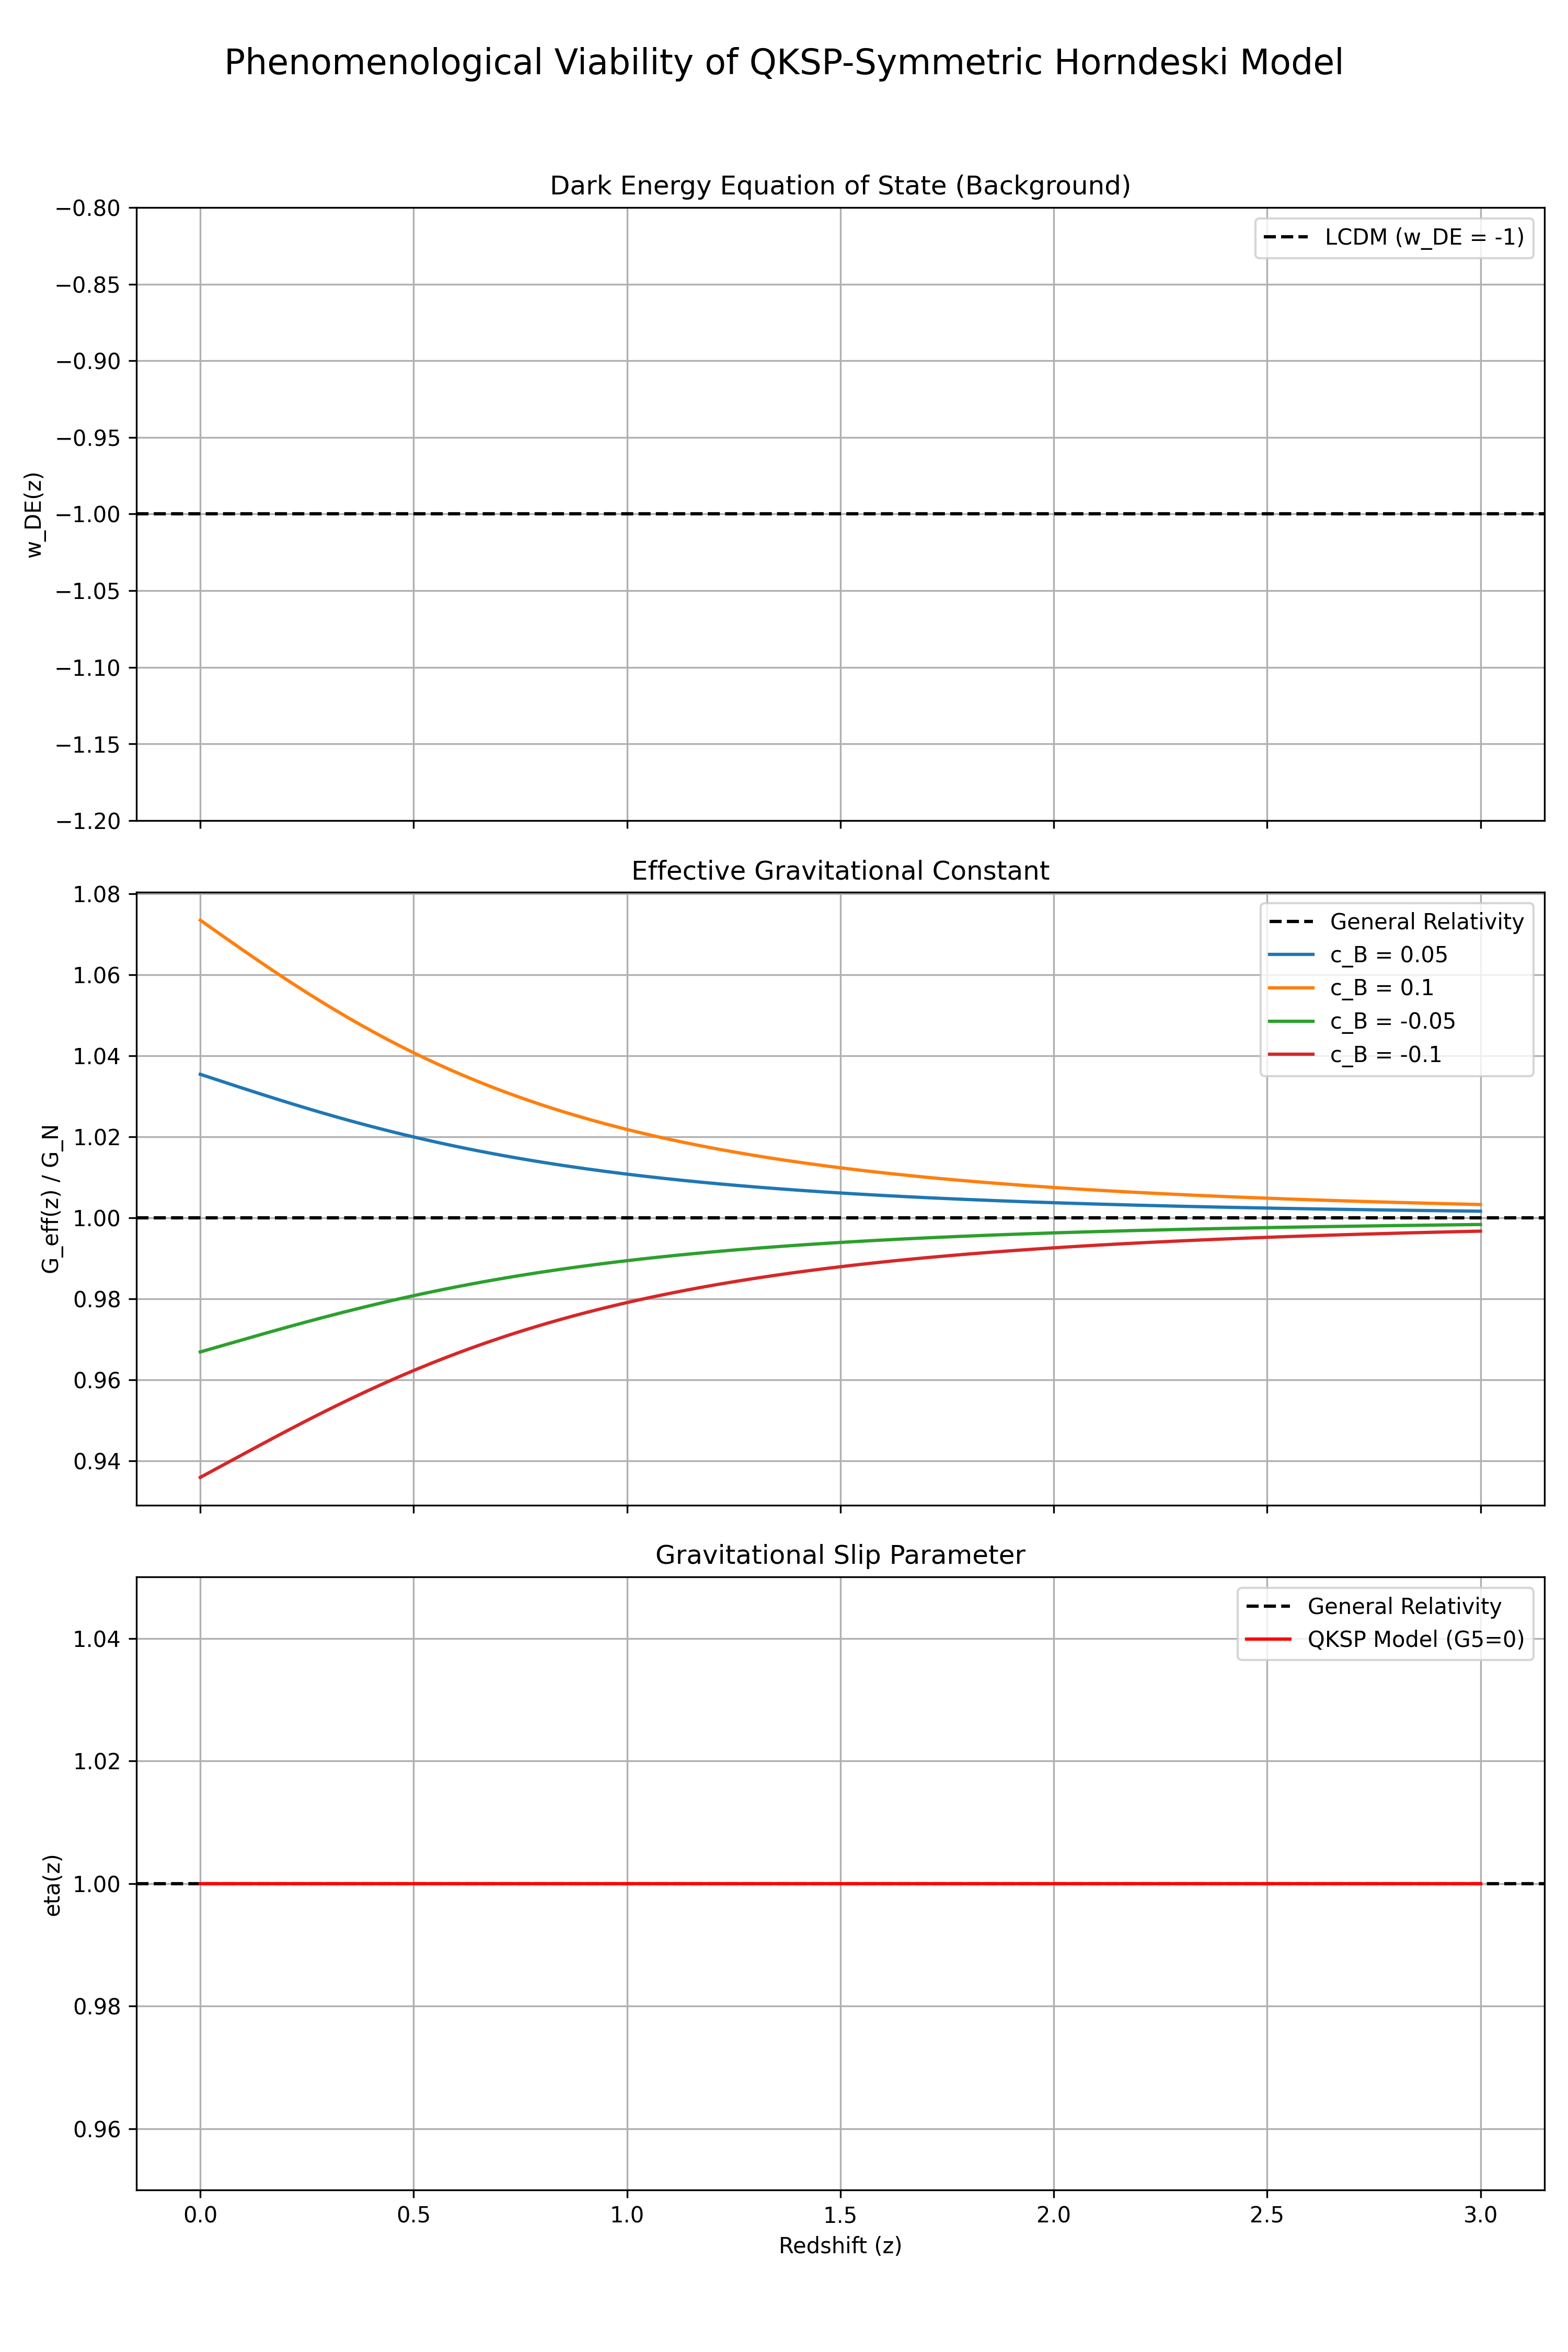
\includegraphics[width=0.5\textwidth]{../input_files/plots/horndeski_phenomenology_plot_1_20250925-220824.png}
    \caption{Cosmological observables for a Quantum Kinetic Structure Preservation (QKSP)-symmetric Horndeski model. Top panel: Dark energy equation of state $w_{DE}(z)$ is fixed at $-1$, consistent with $\Lambda$CDM. Middle panel: Effective gravitational constant $G_{\text{eff}}(z)/G_N$ showing time-dependent deviations from General Relativity for varying braiding parameters $c_B$, with gravity enhanced ($c_B > 0$) or suppressed ($c_B < 0$) at low redshifts. Bottom panel: Gravitational slip parameter $\eta(z)$ remains unity, consistent with General Relativity for models with $G_5=0$. This figure illustrates how the requirement of quantum stability leads to specific, testable modifications in the strength of gravity.}
    \label{fig:horndeski_phenomenology}
\end{figure}

\subsection{Discussion of Results and Future Avenues}
Our results establish a robust connection between fundamental quantum stability requirements and observable cosmological phenomena. The QKSP symmetry, demanding $c_s^2 = c_T^2 = 1$, significantly constrains the vast parameter space of Horndeski theories, yielding a theoretically well-motivated subset.

\subsubsection{Robustness and Generality}
While the phenomenological analysis presented here focused on a specific, well-motivated parameterization ($\alpha_B = c_B \Omega_{DE}$ and $G_5=0$), the underlying QKSP condition, $c_s^2=1$, is a general differential constraint on the Horndeski functions $G_i(\phi, X)$. Future work should explore the broader space of solutions to this condition to understand the full range of possible cosmological dynamics and observable signatures. In particular, investigating QKSP\ensuremath{\_}symmetric models with a non-zero $G_5(\phi)$ is crucial, as such models would typically predict $\eta \neq 1$, offering a second independent observational channel to test these theories against General Relativity.

\subsubsection{Beyond the One-Loop Approximation}
The QKSP principle, as formulated in this work, ensures the absence of ghost instabilities at the one-loop level. A critical theoretical question remains whether this symmetry can protect the theory from the generation of new ghost degrees of freedom at higher loop orders. Proving an "all-orders" non-renormalization theorem for the ghost kinetic term would significantly strengthen the theoretical foundation of QKSP\ensuremath{\_}symmetric theories, solidifying their status as genuinely stable quantum theories of gravity.

\subsubsection{Precision Cosmology and Observational Tests}
Our analysis of $G_{\text{eff}}$ and $\eta$ was conducted using the quasi-static, sub-horizon approximation. For a more rigorous and comprehensive comparison with high-precision cosmological data, especially from the Cosmic Microwave Background (CMB) and large-scale structure, it is essential to implement QKSP\ensuremath{\_}symmetric models into a full numerical Boltzmann solver (e.g., \texttt{CAMB} or \texttt{CLASS}). This would enable the computation of complete power spectra for matter, galaxy clustering, and weak lensing, allowing for a detailed statistical comparison with observational data and precise constraints on the coupling parameter $c_B$. Such an endeavor would represent the next crucial step in testing the viability of this quantum-stable framework.

\section{Conclusions}
\label{sec:conclusions}


\subsection{Problem and Solution}
Modified gravity theories, particularly Horndeski theories, offer a compelling framework to address the mysteries of dark energy and dark matter within the $\Lambda$CDM model. While classically designed to be ghost-free, their stability at the quantum level, where loop corrections can introduce problematic higher-derivative ghost terms, remains a critical challenge. This paper introduced the Quantum Kinetic Structure Preservation (QKSP) symmetry as a novel principle to ensure the one-loop quantum stability of Horndeski theories by explicitly preventing the generation of new propagating ghost degrees of freedom.

\subsection{Methods}
Our methodology involved a multi-stage theoretical and phenomenological analysis. We began by establishing classical stability conditions for Horndeski theories around a flat Friedmann-Lemaître-Robertson-Walker (FLRW) background, incorporating the crucial observational constraint of luminal gravitational wave propagation ($c_T^2=1$). The one-loop effective action was then rigorously computed using the background field method and heat kernel regularization to identify quantum-generated higher-derivative terms. The QKSP conditions were derived by demanding the vanishing of coefficients for terms that would introduce higher-than-second-order time derivatives in the effective action for physical perturbations. Finally, a representative QKSP-symmetric model, capable of mimicking the $\Lambda$CDM expansion history, was subjected to a phenomenological analysis to assess its observational signatures, specifically focusing on the effective gravitational constant ($G_{\text{eff}}$) and the gravitational slip parameter ($\eta$).

\subsection{Results}
The theoretical cornerstone of this work is the QKSP symmetry, which fundamentally implies that scalar and tensor modes must propagate at the same speed ($c_s^2 = c_T^2$) to maintain quantum stability at the one-loop level. Combined with the robust observational constraint $c_T^2=1$, this leads to the strong and direct prediction that QKSP-symmetric Horndeski theories must satisfy $c_s^2=1$. This establishes a profound link between fundamental quantum requirements and the causal structure of cosmological perturbations. Our phenomenological investigation of a QKSP-symmetric model, chosen to reproduce the $\Lambda$CDM background expansion and with $G_5=0$, revealed that such theories predict a gravitational slip parameter $\eta=1$, similar to General Relativity. However, they exhibit time-dependent modifications to the effective gravitational constant, $G_{\text{eff}}$. For example, a coupling parameter $|c_B|=0.1$ predicts percent-level deviations in $G_{\text{eff}}$ (e.g., a 7.4\% enhancement or 6.4\% suppression at $z=0$) that are within the detection capabilities of current and future large-scale structure surveys.

\subsection{What We Have Learned}
This work demonstrates that fundamental quantum stability requirements can impose stringent and testable constraints on modified gravity theories. The QKSP symmetry provides a robust theoretical framework for building quantum-stable Horndeski models, significantly narrowing down the vast parameter space of possible theories. The derived prediction $c_s^2=1$ is a powerful, universal consequence of quantum stability in this context. Furthermore, we have shown that even a simplified QKSP-symmetric model, mimicking $\Lambda$CDM expansion and without gravitational slip, offers distinct and falsifiable predictions for the growth of cosmic structures via $G_{\text{eff}}$. These deviations are within reach of upcoming cosmological surveys, establishing a direct and testable bridge between fundamental quantum principles and observable cosmological phenomena. Future research should explore the broader landscape of QKSP-symmetric models, investigate higher-order loop stability, and integrate these models into full Boltzmann solvers for precise observational comparisons.

\bibliography{bibliography}{}
\bibliographystyle{aasjournal}

\end{document}
